\section{Results}

\begin{figure}[ht]
  \begin{center}
      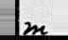
\includegraphics[width=0.09\textwidth]{images/Subimages/Good/004531795_00006-3.png}
      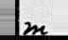
\includegraphics[width=0.09\textwidth]{images/Subimages/Good/004531795_00006-3.png}
      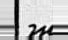
\includegraphics[width=0.09\textwidth]{images/Subimages/Good/004531795_00006-5.png}
      
\includegraphics[width=0.09\textwidth]{images/Subimages/Good/004531795_00009-60.png}
      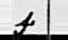
\includegraphics[width=0.09\textwidth]{images/Subimages/Good/004531795_00009-80.png}
      
\includegraphics[width=0.09\textwidth]{images/Subimages/Good/004531795_00195-67.png}
      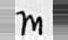
\includegraphics[width=0.09\textwidth]{images/Subimages/Good/004531795_00195-72.png}
      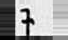
\includegraphics[width=0.09\textwidth]{images/Subimages/Good/004531795_00195-91.png}
      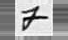
\includegraphics[width=0.09\textwidth]{images/Subimages/Good/004531795_00439-74.png}
      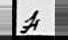
\includegraphics[width=0.09\textwidth]{images/Subimages/Good/004531795_00009-59.png}
    \\[1em]
      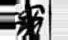
\includegraphics[width=0.09\textwidth]{images/Subimages/problematic/004531795_00275-72.png}
      
\includegraphics[width=0.09\textwidth]{images/Subimages/problematic/004531795_00275-86.png}
      
\includegraphics[width=0.09\textwidth]{images/Subimages/problematic/004531795_00276-2.png}
      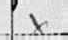
\includegraphics[width=0.09\textwidth]{images/Subimages/problematic/004531795_00276-49.png}
      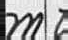
\includegraphics[width=0.09\textwidth]{images/Subimages/problematic/004531795_00605-8.png}
      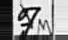
\includegraphics[width=0.09\textwidth]{images/Subimages/problematic/004531795_00778-55.png}
      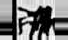
\includegraphics[width=0.09\textwidth]{images/Subimages/problematic/004531871_00823-56.png}
  \end{center}
  \caption{
    Top row: examples of good images extracted from the LDS dataset.
    Bottom row: examples of noise from the LDS dataset.
    }
  \label{fig:goodAndBad}
\end{figure}

The data we used, even after cleaning, was not entirely clean.  As can be seen in Figure~\ref{fig:goodAndBad}, we had many good images, that were expanded to be a uniform size.  But we had images where the field was crossed out, or even bounding boxes that covered completely different columns, or having data from multiple columns.  The images seen in that figure are representative of the dataset passed to our classifier.  We had a total of approximately 70,000 examples to split up into training, testing, and verification data sets.

We first implemented linear classifiers and trained them on our image data.  The Averaged Perceptron performed well with a cross-validation accuracy of 81.3\%, and test accuracy of 81.85\%.  The SVM classifier performed a little worse with cross-validation accuracy of 78.9\%, and test accuracy of 80.3\%.  This was a surprising result due to the expected non-linearity of our input data.

After classifying with linear classifiers, we ran the CNN classifier using two convolutional layers and a logistic regression multi-layered perceptron at the end.  We performed cross-validation to determine the learning rate and the two kernel parameters determining how many convolutions to perform at each of the convolution layers.  The best parameters were consistently $r = 0.05$, $k_1 = 20$, and $k_2 = 50$.  A plot of the accuracy on the validation set can be seen in Figure~\ref{fig:valAccuracyDuringTraining}.  The cross-validation and training took nearly 6 hours to perform.  The cross-validation accuracy was 88.6\%, and can be seen in Table~\ref{tbl:cnnCrossVal}.  The test accuracy after training was 96.1\%.  We were very surprised by this result considering the noise we still have in our data.

%\begin{table}[h]
%  \caption{Average over all cross-validation runs for (left) Averaged Perceptron and (right) SVM}
%  \label{tbl:avgPerceptronCrossVal}
%  \begin{center}
%    \begin{tabular}{|c|c|c|}
%      \hline
%        r    & Test Accuracy   & Train Accuracy   \\
%      \hline
%      0.0001 &      0.814      &      0.817       \\
%      0.001  &      0.802      &      0.806       \\
%      0.010  &      0.813      &      0.816       \\
%      0.100  &      0.799      &      0.804       \\
%      0.500  &      0.813      &      0.817       \\
%      \hline
%    \end{tabular}
%    \begin{tabular}{|c|c|c|c|}
%      \hline
%        r   &    C   & Test Accuracy   & Train Accuracy  \\
%      \hline
%      0.010 &  0.000 &      0.747      &      0.757        \\
%      0.010 &  0.100 &      0.762      &      0.769        \\
%      0.100 &  0.001 &      0.778      &      0.781        \\
%      0.100 &  0.010 &      0.789      &      0.796        \\
%      0.500 &  0.100 &      0.775      &      0.782        \\
%      \hline
%    \end{tabular}
%  \end{center}
%\end{table}
%Using the results r=.0001 the total accuracy with our test set =   81.85
%
%For SVM we got the following results:
\begin{table}[h]
  \caption{Average over all cross-validation runs}
  \label{tbl:cnnCrossVal}
  \begin{center}
    \begin{tabular}{|c|c|c|c|c|}
      \hline
        r   &   k1 & k2 & Test Accuracy   & Train Accuracy  \\
      \hline
      0.100 &   10 & 20 &      0.786      &      0.788      \\  
      0.100 &   10 & 50 &      0.801      &      0.803      \\  
      0.100 &   20 & 20 &      0.790      &      0.794      \\  
      0.100 &   20 & 50 &      0.622      &      0.628      \\  
      0.050 &   10 & 20 &      0.747      &      0.748      \\  
      0.050 &   10 & 50 &      0.861      &      0.861      \\  
      0.050 &   20 & 20 &      0.804      &      0.804      \\  
      0.050 &   20 & 50 &      0.886      &      0.888      \\  
      0.010 &   10 & 20 &      0.792      &      0.791      \\  
      0.010 &   10 & 50 &      0.815      &      0.818      \\  
      0.010 &   20 & 20 &      0.748      &      0.750      \\  
      0.010 &   20 & 50 &      0.800      &      0.800      \\  
      0.005 &   10 & 20 &      0.706      &      0.707      \\  
      0.005 &   10 & 50 &      0.768      &      0.772      \\  
      0.005 &   20 & 20 &      0.642      &      0.645      \\  
      0.005 &   20 & 50 &      0.716      &      0.717      \\  
      \hline
    \end{tabular}
  \end{center}
\end{table}
%Using the result $r=.1$ and $C= .01$ the total accuracy with our test set = test accuracy: $0.803083291699$

\begin{figure}[ht]
  \centering
  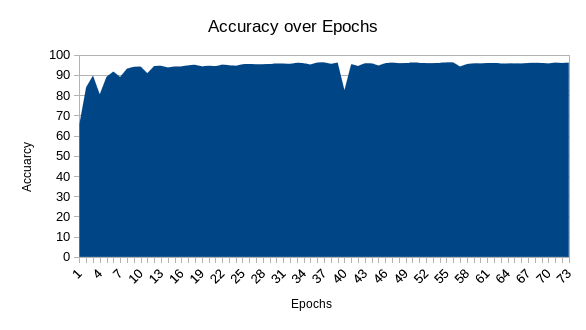
\includegraphics[width=0.7\textwidth]{images/AccuracyoverEpochslog7.png}
  \caption{
    Validation accuracy recorded during training of the CNN classifier on the
    LDS dataset for gender
    }
  \label{fig:valAccuracyDuringTraining}
\end{figure}




